\begin{appendix}
\chapter{Résultats des traitements d'images}
\section{Sous-échantillonnages} \label{annexe.traitement.downsampling}

\begin{figure}[H]
    \centering
    \begin{subfigure}{.4\textwidth}
        \centering
        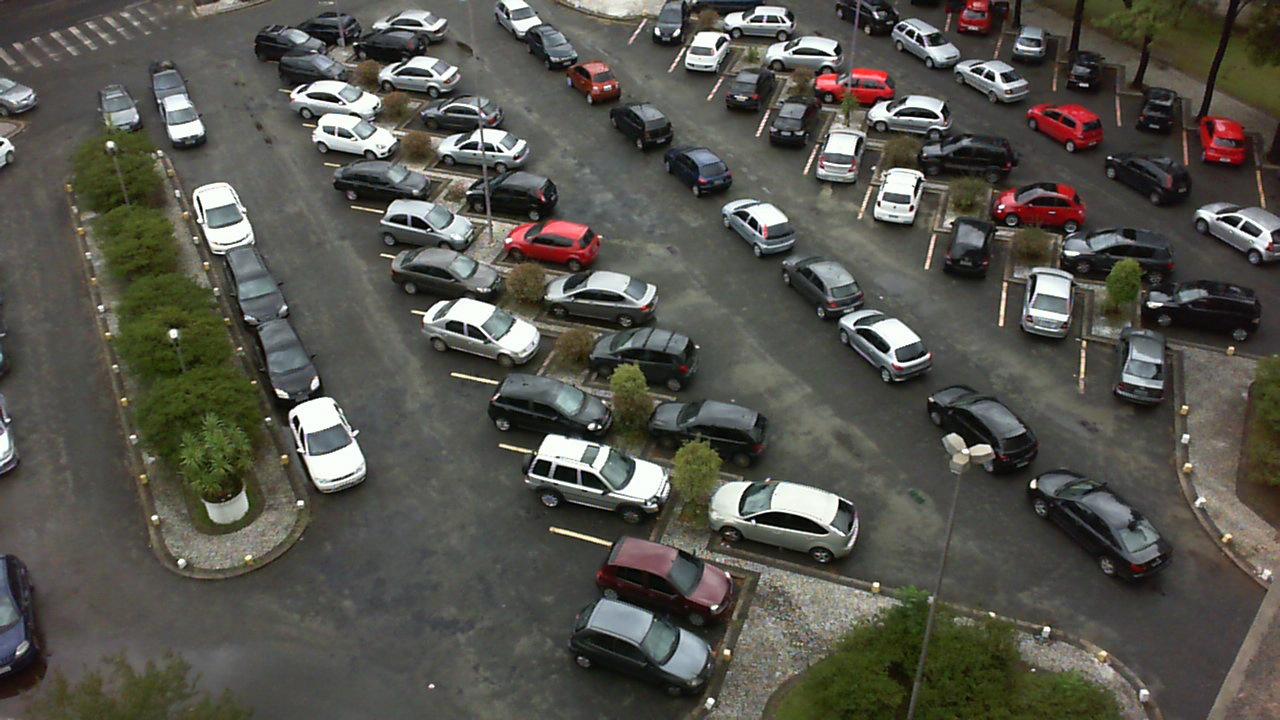
\includegraphics[width=.85\linewidth]{img/conception/image_process/downsample_only/7.png}
        \caption{1280 x 720}
    \end{subfigure}%
    \begin{subfigure}{.4\textwidth}
        \centering
        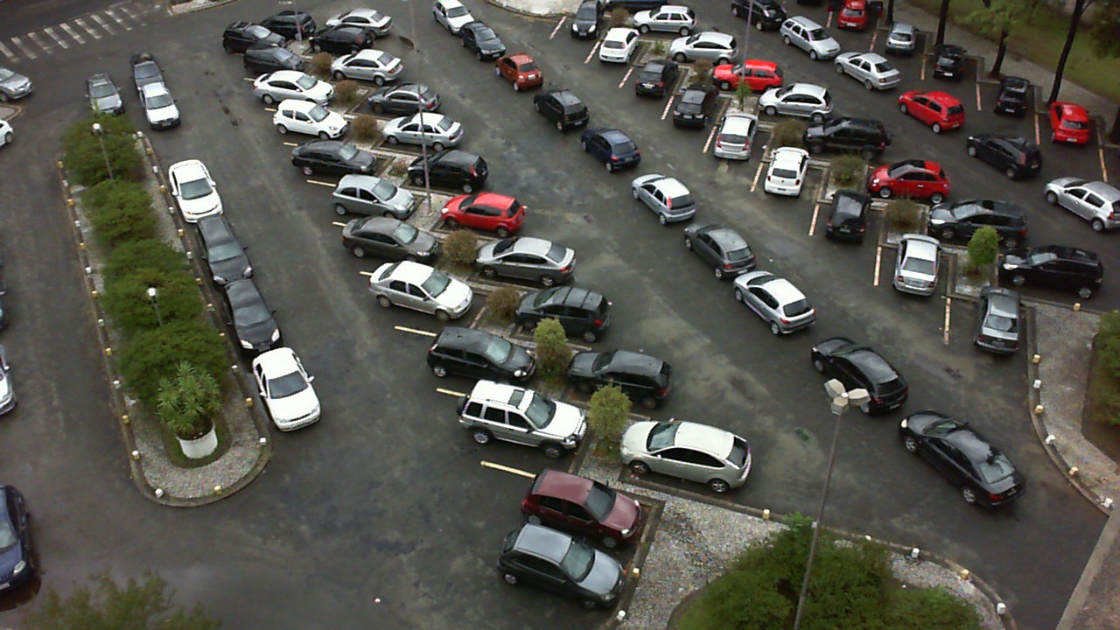
\includegraphics[width=.85\linewidth]{img/conception/image_process/downsample_only/6.png}
        \caption{1120 x 630}
    \end{subfigure}%   

    \bigskip
    \begin{subfigure}{.4\textwidth}
        \centering
        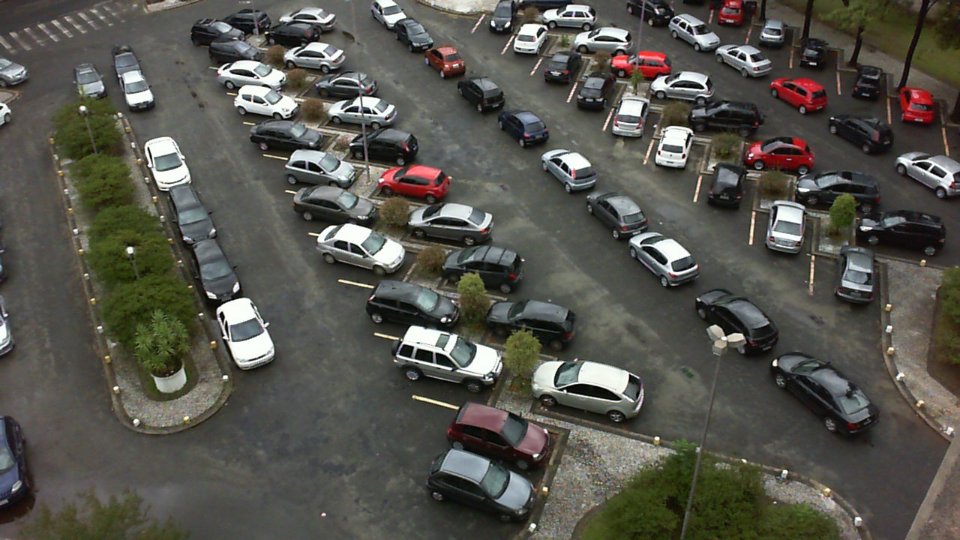
\includegraphics[width=.85\linewidth]{img/conception/image_process/downsample_only/5.png}
        \caption{960 x 540}   
    \end{subfigure}%   
    \begin{subfigure}{.4\textwidth}
        \centering
        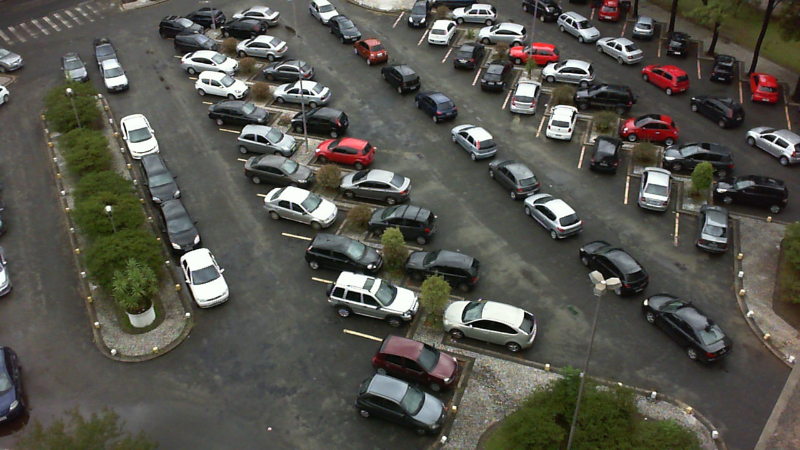
\includegraphics[width=.85\linewidth]{img/conception/image_process/downsample_only/4.png}
        \caption{800 x 450}
    \end{subfigure}% 

    \bigskip
    \begin{subfigure}{.4\textwidth}
        \centering
        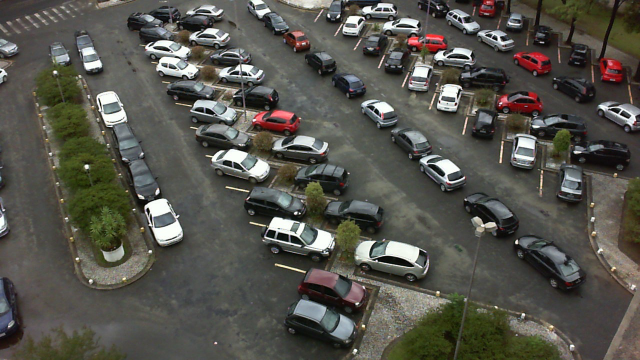
\includegraphics[width=.85\linewidth]{img/conception/image_process/downsample_only/3.png}
        \caption{640 x 360}
    \end{subfigure}%   
    \begin{subfigure}{.4\textwidth}
        \centering
        
\includegraphics[width=.85\linewidth]{img/conception/image_process/downsample_only/2.png}
        \caption{480 x 270}
    \end{subfigure}%  

    \bigskip
    \begin{subfigure}{.4\textwidth}
        \centering
        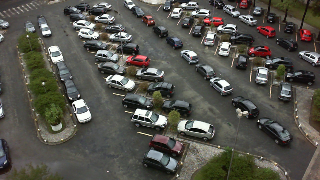
\includegraphics[width=.85\linewidth]{img/conception/image_process/downsample_only/1.png}
        \caption{320 x 180}
    \end{subfigure}%   
    \begin{subfigure}{.4\textwidth}
        \centering
        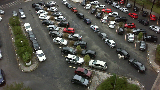
\includegraphics[width=.85\linewidth]{img/conception/image_process/downsample_only/0.png}
        \caption{160 x 90}
    \end{subfigure}%   
    \caption{L'image originale redimensionnée à différentes résolutions}
\end{figure}

\section{Détection de bords, sous-échantillonnage} \label{annexe.traitement.edge_down}
Ici, il est considéré que la détection de bord a été effectuée en premier, à l'aide d'un filtre \textit{Scharr} est appliqué sur l'espace HSV de l'image.

\begin{figure}[H]
    
\includegraphics[width=80mm]{img/conception/image_process/edges_only/5.png}
    \centering
    \caption{\textit{Scharr} HSV: image utilisée afin d'explorer les différents sous-échantillonnages}
    \label{fig:image_process_edge_down_orig}
\end{figure}

\begin{figure}[H]
    \begin{subfigure}{.5\textwidth}
        \centering
        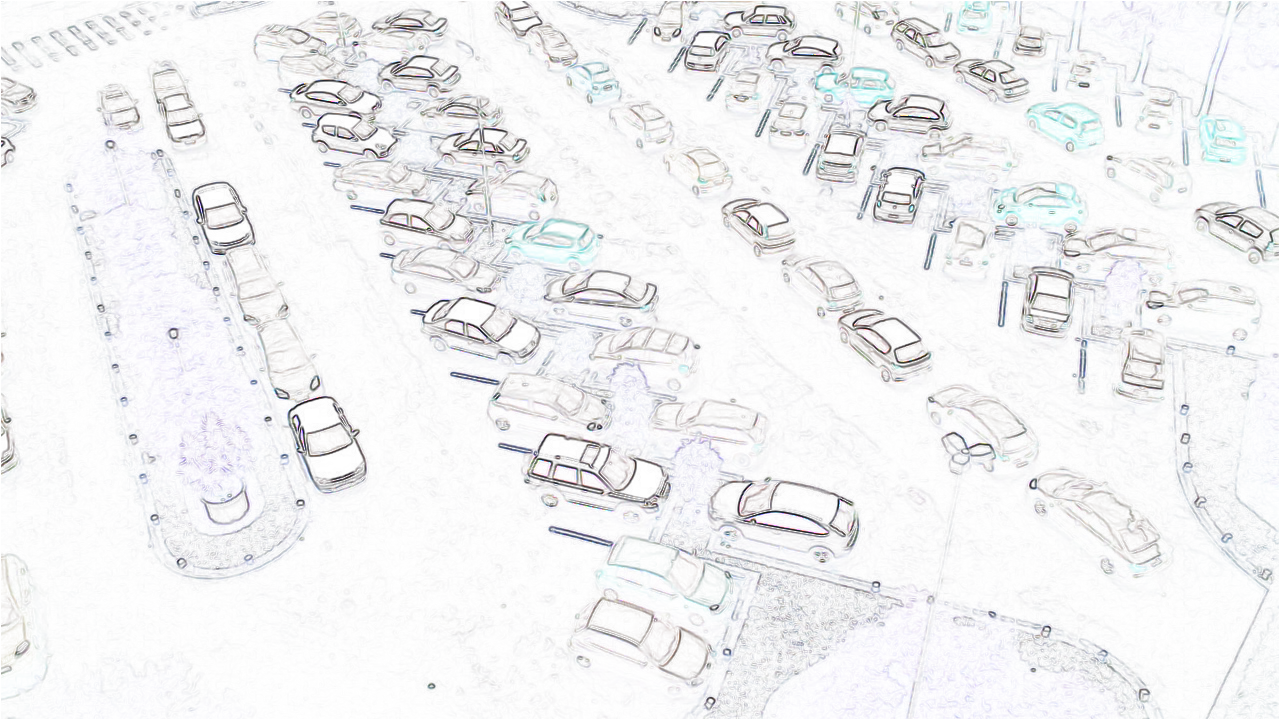
\includegraphics[width=.85\linewidth]{img/conception/image_process/edge-downsample/7.png}
        \caption{1280 x 720}
    \end{subfigure}%
    \begin{subfigure}{.5\textwidth}
        \centering
        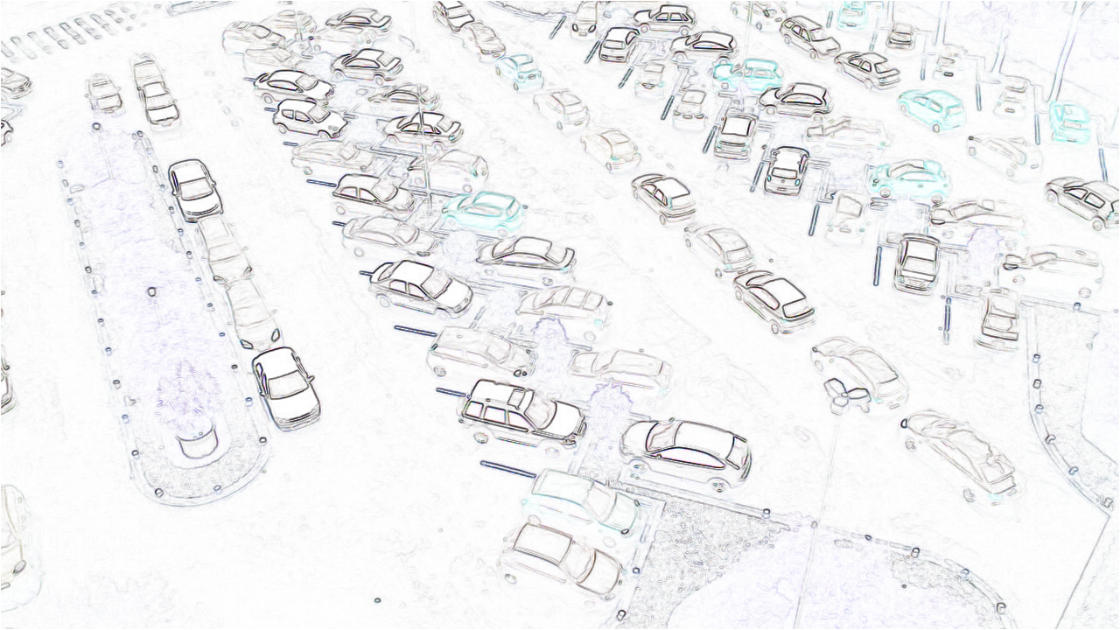
\includegraphics[width=.85\linewidth]{img/conception/image_process/edge-downsample/6.png}
        \caption{1120 x 630}
    \end{subfigure}%   

    \bigskip
    \begin{subfigure}{.5\textwidth}
        \centering
        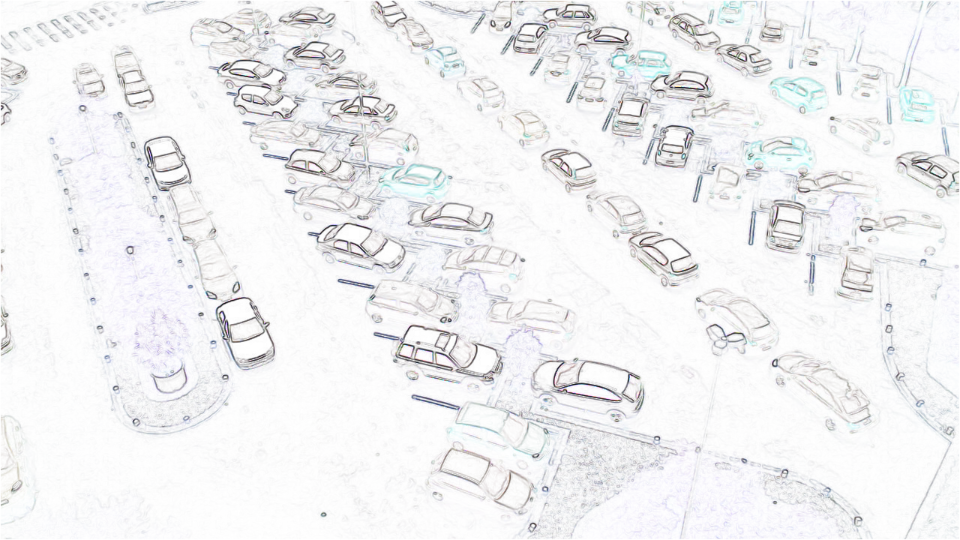
\includegraphics[width=.85\linewidth]{img/conception/image_process/edge-downsample/5.png}
        \caption{960 x 540}   
    \end{subfigure}%   
    \begin{subfigure}{.5\textwidth}
        \centering
        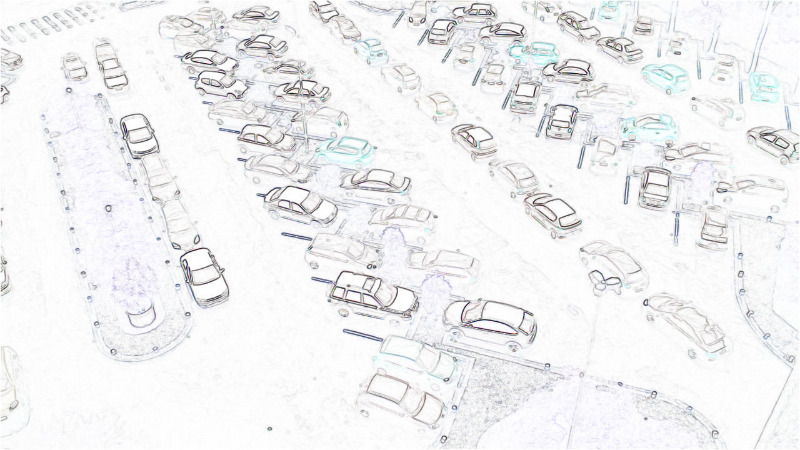
\includegraphics[width=.85\linewidth]{img/conception/image_process/edge-downsample/4.png}
        \caption{800 x 450}
    \end{subfigure}% 

    \bigskip
    \begin{subfigure}{.5\textwidth}
        \centering
        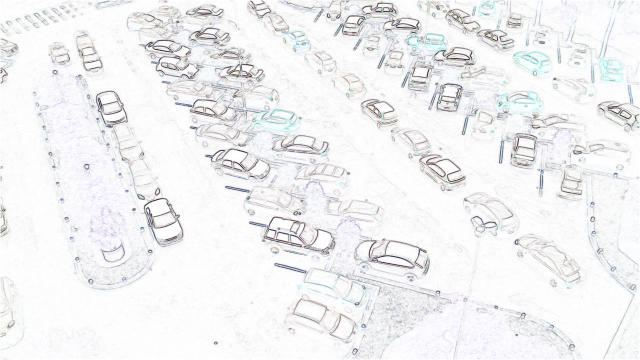
\includegraphics[width=.85\linewidth]{img/conception/image_process/edge-downsample/3.png}
        \caption{640 x 360}
    \end{subfigure}%   
    \begin{subfigure}{.5\textwidth}
        \centering
        
\includegraphics[width=.85\linewidth]{img/conception/image_process/edge-downsample/2.png}
        \caption{480 x 270}
    \end{subfigure}%  
    
    \bigskip
    \begin{subfigure}{.5\textwidth}
        \centering
        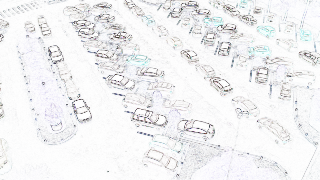
\includegraphics[width=.85\linewidth]{img/conception/image_process/edge-downsample/1.png}
        \caption{320 x 180}
    \end{subfigure}%   
    \begin{subfigure}{.5\textwidth}
        \centering
        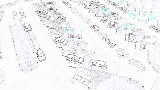
\includegraphics[width=.85\linewidth]{img/conception/image_process/edge-downsample/0.png}
        \caption{160 x 90}
    \end{subfigure}%   
    \centering
    \caption{L'image dont les bords ont été détectés, redimensionnée à différentes résolutions}
    \label{fig:image_process_edge_down}
\end{figure}

La figure \ref{fig:image_process_edge_down} applique plusieurs sous-échantillonnages de l'image \ref{fig:image_process_edge_down_orig}.

Il semble que l'image la plus légère et suffisamment précise afin de pouvoir détecter sans encombre des voitures est celle dont la résolution est de 480 x 270 pixels. Les images dont la taille est inférieure sont trop floues, où certaines voitures semblent parfois même disparaitre.


\section{Détection de bords, sous-échantillonnage} \label{annexe.traitement.down_edge}

Ce paragraphe présente les résultats d'un traitement qui consiste en sous-échantillonner l'image dans un premier temps, puis d'en détecter les bords. Lors des différents tests effectués, il a été remarqué qu'une résolution de 320x180 pixels, tel qu'indiqué dans le paragraphe \itnameref{conception.traitement.eval.downsample}, ne produisait pas des résultats concluants. C'est pourquoi la résolution de 480 x 270 pixels a été préférée. L'image utilisée est présentée en figure \ref{fig:image_process_down_edge_orig}.

\begin{figure}[H]
    
\includegraphics[width=110mm]{img/conception/image_process/downsample_only/2.png}
    \centering
    \caption{480 x 270: image utilisée afin d'explorer les différentes méthodes de détection de bords}
    \label{fig:image_process_down_edge_orig}
\end{figure}

\begin{figure}[H]
    \begin{subfigure}{.5\textwidth}
        \centering
        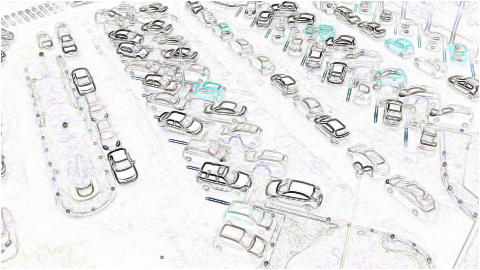
\includegraphics[width=.85\linewidth]{img/conception/image_process/downsample-edge/0.png}
        \caption{Filtre \textit{Sobel} - RGB}
    \end{subfigure}%   
    \begin{subfigure}{.5\textwidth}
        \centering
        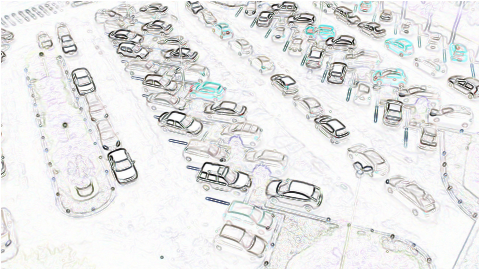
\includegraphics[width=.85\linewidth]{img/conception/image_process/downsample-edge/3.png}
        \caption{Filtre \textit{Scharr} - RGB}
    \end{subfigure}%  

    \bigskip
    \begin{subfigure}{.5\textwidth}
        \centering
        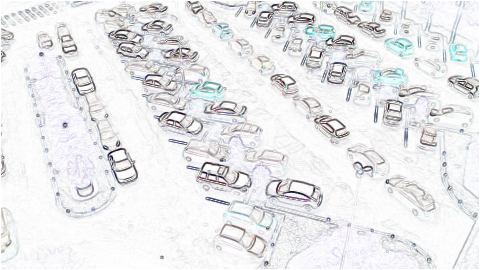
\includegraphics[width=.85\linewidth]{img/conception/image_process/downsample-edge/1.png}
        \caption{Filtre \textit{Sobel} - HSV}   
    \end{subfigure}%   
    \begin{subfigure}{.5\textwidth}
        \centering
        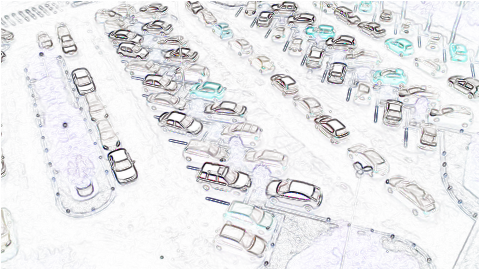
\includegraphics[width=.85\linewidth]{img/conception/image_process/downsample-edge/4.png}
        \caption{Filtre \textit{Scharr} - HSV}
    \end{subfigure}% 
    
    \bigskip
    \begin{subfigure}{.5\textwidth}
        \centering
        
\includegraphics[width=.85\linewidth]{img/conception/image_process/downsample-edge/2.png}
        \caption{Filtre \textit{Sobel} - Valeurs de gris}
    \end{subfigure}%   
    \begin{subfigure}{.5\textwidth}
        \centering
        
\includegraphics[width=.85\linewidth]{img/conception/image_process/downsample-edge/5.png}
        \caption{Filtre \textit{Scharr} - Valeurs de gris}
    \end{subfigure}%   
    \centering
    \caption{L'image sous-échantillonnée avec différentes détections de bords}
    \label{fig:image_process_down_edge}
\end{figure}

La figure \ref{fig:image_process_down_edge} présente l'application des différents filtres sur l'image sous-échantillonnées

Ici, de la même manière que décrit en annexe précédente \itnameref{annexe.traitement.down_edge}, le filtre semblant le mieux convenir est la matrice de convolution définie par \textit{Scharr} sur l'espace HSV. Les voitures y sont mieux distinguables, notamment grâce à leurs couleurs.

\chapter{Planifications}
\todo{Planif}

\end{appendix}